\PassOptionsToPackage{unicode}{hyperref}
\PassOptionsToPackage{hyphens}{url}
\documentclass{article}
\setcounter{secnumdepth}{3}

\usepackage{amsmath,amssymb}
\usepackage{lmodern}
\usepackage{iftex}
\usepackage[letterpaper, margin=1in, top=0.5in, bottom=1in]{geometry}
\usepackage{listings}
\usepackage{color}
\usepackage{titling}
\usepackage{graphicx}
\usepackage{hyperref}

\ifPDFTeX
  \usepackage[T1]{fontenc}
  \usepackage[utf8]{inputenc}
  \usepackage{textcomp} 
\else 
  \usepackage{unicode-math}
  \defaultfontfeatures{Scale=MatchLowercase}
  \defaultfontfeatures[\rmfamily]{Ligatures=TeX,Scale=1}
\fi
\IfFileExists{upquote.sty}{\usepackage{upquote}}{}
\IfFileExists{microtype.sty}{
  \usepackage[]{microtype}
  \UseMicrotypeSet[protrusion]{basicmath} 
}{}
\makeatletter
\@ifundefined{KOMAClassName}{
  \IfFileExists{parskip.sty}{
    \usepackage{parskip}
  }{
    \setlength{\parindent}{0pt}
    \setlength{\parskip}{6pt plus 2pt 2pt}}
}{
  \KOMAoptions{parskip=half}}
\makeatother
\usepackage{xcolor}
\usepackage{graphicx}

\makeatletter
\def\maxwidth{\ifdim\Gin@nat@width>\linewidth\linewidth\else\Gin@nat@width\fi}
\def\maxheight{\ifdim\Gin@nat@height>\textheight\textheight\else\Gin@nat@height\fi}
\makeatother
\setkeys{Gin}{width=\maxwidth,height=\maxheight,keepaspectratio}
\makeatletter
\def\fps@figure{htbp}
\makeatother
\setlength{\emergencystretch}{3em} 
\providecommand{\tightlist}{
  \setlength{\itemsep}{0pt}\setlength{\parskip}{0pt}}

\ifLuaTeX
  \usepackage{selnolig}  
\fi
\IfFileExists{bookmark.sty}{\usepackage{bookmark}}{\usepackage{hyperref}}
\IfFileExists{xurl.sty}{\usepackage{xurl}}{} 
\urlstyle{same}
\hypersetup{
  hidelinks,
  pdfcreator={LaTeX via pandoc}}

\title{Artifacts - Sprint 1}
\date{}

\begin{document}

\maketitle

\hypertarget{sos-s1} {
\section{Scrum of Scrums}\label{Scrum of Scrums} 
During this 1st sprint, the team had started to define and implement the initial contract 
for the developer. So, some of the most important User Stories were #18 and #30. On the other hand, 
the team also started to prioritize User Stories #19 and #20 to complete the game execution.
All of the above User Stories mentioned had a special discussion in the Lead's Daily that
occurred on Tuesday and Thursday, due to see the approaches for the contract 
and the graphic library to be difined for the game execution needed.
}

\href{https://tree.taiga.io/project/joseluis-teran-coffeetime/taskboard/sprint-1-9301}{Link: User Stories of Sprint 1 on Taiga}.

\begin{figure}
\centering
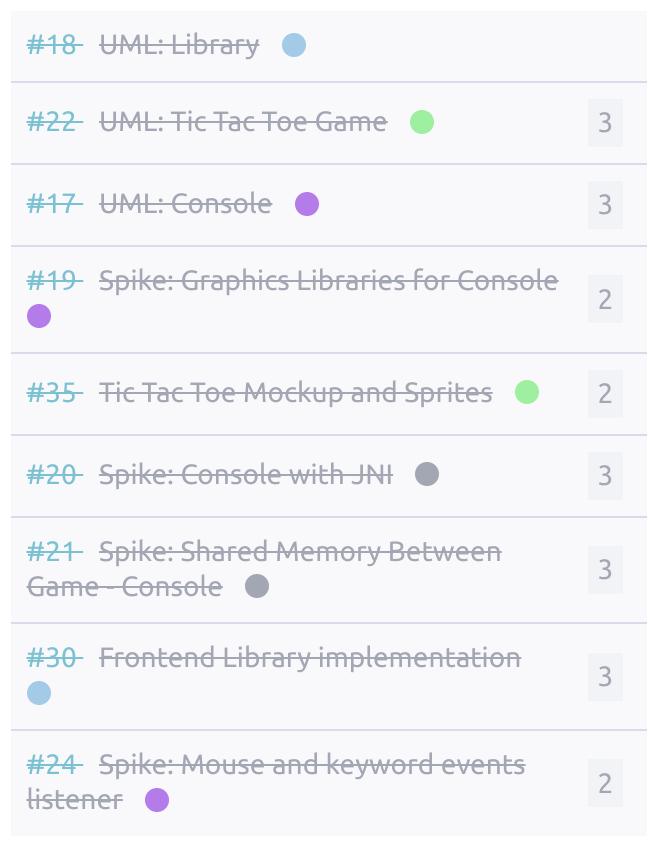
\includegraphics[width=8cm, height=15cm]{./assets/us-s1.png}
\end{figure}

\hypertarget{burndownchart-s1}{
\section{Burn Down Chart}\label{Burn Down Chart S1}}
\href{https://tree.taiga.io/project/joseluis-teran-coffeetime/taskboard/sprint-1-9301}{Link: Sprint 1 Board on Taiga}.

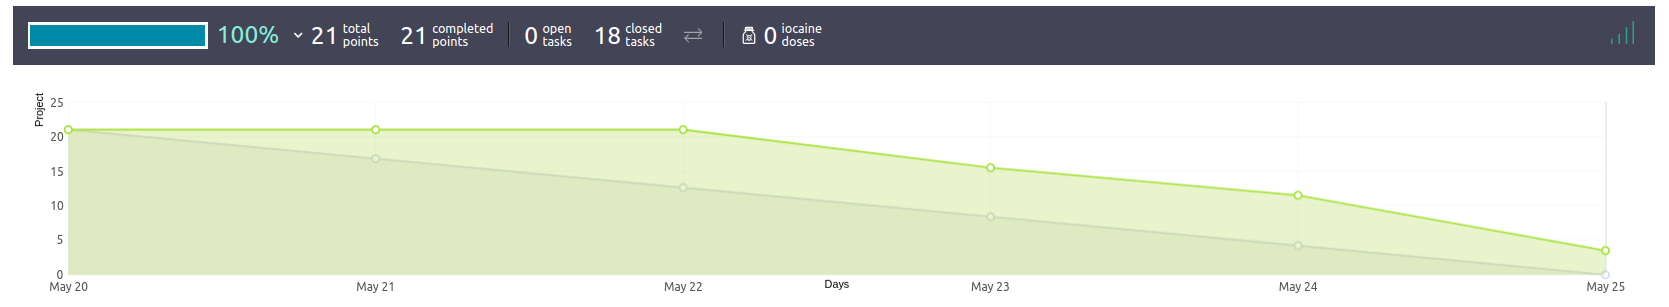
\includegraphics[width=\textwidth]{./assets/burndown-s1.png}

\hypertarget{startstopcontinueactionitems-s1}{
\section{Start-Stop-Continue-Action Items}\label{Start-Stop-Continue-Action Items S1}}
\href{https://miro.com/app/board/uXjVKDO7l8M=/?moveToWidget=3458764590247693119&cot=14}{Link: Start-Stop-Continue-Action Items Sprint 1 on Miro}.

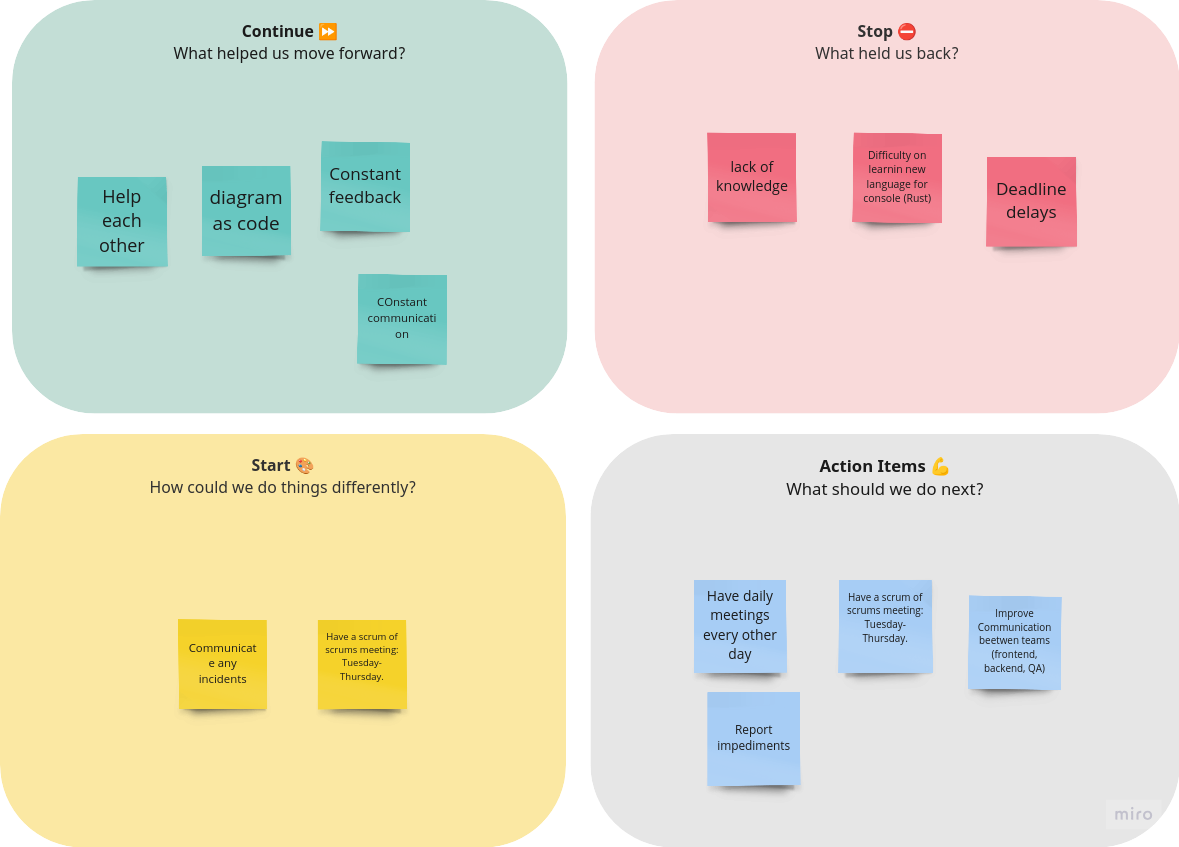
\includegraphics[width=\textwidth]{./assets/retrospective-s1.png}

\end{document}
